\documentclass[dvipsnames,a4paper,11pt]{article}
\usepackage[brazil]{babel}
\usepackage[T1]{fontenc}
\usepackage[utf8x]{inputenc}
\usepackage{graphicx}
\usepackage{hyperref}
\usepackage{amssymb}
\usepackage{color}
\usepackage{amsmath}
\usepackage{listings} 
\usepackage[section]{placeins}

% You can include more LaTeX packages here 

\definecolor{mygreen}{rgb}{0,0.6,0}
\definecolor{mygray}{rgb}{0.5,0.5,0.5}
\definecolor{mymauve}{rgb}{0.58,0,0.82}

\lstset{ %
	backgroundcolor=\color{white},   % choose the background color; you must add \usepackage{color} or \usepackage{xcolor}
	basicstyle=\small,        % the size of the fonts that are used for the code
	breakatwhitespace=false,         % sets if automatic breaks should only happen at whitespace
	breaklines=true,                 % sets automatic line breaking
	captionpos=b,                    % sets the caption-position to bottom
	commentstyle=\color{mygreen},    % comment style
	escapeinside={\%*}{*)},          % if you want to add LaTeX within your code
	extendedchars=true,              % lets you use non-ASCII characters; for 8-bits encodings only, does not work with UTF-8
	keepspaces=true,                 % keeps spaces in text, useful for keeping indentation of code (possibly needs columns=flexible)
	keywordstyle=\color{blue},       % keyword style
	language=Python,                 	   % the language of the code
	numbers=left,                    % where to put the line-numbers; possible values are (none, left, right)
	numbersep=5pt,                   % how far the line-numbers are from the code
	numberstyle=\tiny\color{mygray}, % the style that is used for the line-numbers
	rulecolor=\color{black},         % if not set, the frame-color may be changed on line-breaks within not-black text (e.g. comments (green here))
	showspaces=false,                % show spaces everywhere adding particular underscores; it overrides 'showstringspaces'
	showstringspaces=false,          % underline spaces within strings only
	showtabs=false,                  % show tabs within strings adding particular underscores
	%  stepnumber=2,                    % the step between two line-numbers. If it's 1, each line will be numbered
	stringstyle=\color{mymauve},     % string literal style
	tabsize=2,	                   % sets default tabsize to 2 spaces
	title=\lstname                   % show the filename of files included with \lstinputlisting; also try caption instead of title
}

\usepackage[a4paper,top=2.5cm,bottom=2.5cm,left=3cm,right=3cm,marginparwidth=1.75cm]{geometry}

\begin{document}

%\selectlanguage{english} %%% remove comment delimiter ('%') and select language if required

\author{Bruno da silva}

\fontfamily{phv}\selectfont
\begin{titlepage}
	\begin{center}
		{\scshape\Large Universidade Federal Fluminense -UFF \par}
		\vspace{7cm}
		{\huge\bfseries Pendulo forçado \par}
		\vspace{5.5cm}
		{\itshape Autor Bruno da Silva Machado \par}      
			
		\vspace{6.5cm}    
			
		\vfill
		{\large \today\par}
	\end{center}
\end{titlepage}

\setcounter{secnumdepth}{0}
\section{Introdu\c{c}\~{a}o}
\noindent

Em  um sistema vibratório livre quando é posto a oscilar executa um movimento oscilatório próprio. Com sua frequência angular característica determinada apenas pelas propriedades do sistema, entretanto, se é submetido a uma força externa harmônica, ele conserva a maior parte de sua individualidade ligeiramente modificada, devido à presença da força externa harmônica. Portanto, sua frequência é algo diferente do que seria sem estimulação exterior e sua amplitude é modulada no tempo. Esta narrativa descreve um pendulo amortecido forçado que sera e nosso objeto de estudo.
\noindent \eject 

\section{Pendulo Forçado}
\noindent 

A evolução temporal de um sistema dinâmico dissipativo apresenta um atrator: trajetória típica da evolução de um sistema dinâmico para um conjunto definido de parâmetros. Um exemplo bem evidente de sistema dissipativo é o pêndulo amortecido que nesse caso, o atrator era do tipo ponto fixo: qualquer conjunto de condições iniciais leva o sistema a um único ponto no espaço de fase.  
No entanto, um sistema dissipativo pode ser alimentado pela ação de uma força externa que lhe reponha a energia. Nesse caso, o atrator não será necessariamente um ponto fixo. movimentos com essas características podem ter um comportamento periódico ou harmônico, quase-periódico (pseudo-harmônico) ou caótico.  Se o comportamento for periódico, poderá apresentar um atrator do tipo "ciclo limite ". O comportamento quase-periódico determina outros tipos de atratores. Para certos parâmetros poderá ter comportamento caótico, cujo atrator é do tipo estranho. É o que acontece com o Pêndulo Amortecido Forçado.


\begin{center}
	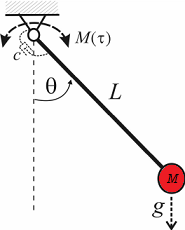
\includegraphics[width=1.85in,height=2.30in,keepaspectratio = false]{nonlinear-pendulum.png}
	
	\scriptsize Figura 1.Pendulo amortecido em movimento com uma força externa sendo aplicado na base da haste do pendulo. 
	
\end{center}

Introduzindo ao pêndulo amortecido o torque de uma força periódica $F = F_0\sin(\omega_D{t})$, onde $\omega_D{t}$ é a frequência angular da força externa, a segunda lei de Newton para rotação deste movimento torna-se:

\[	ml^2\ddot{\theta} = lF_0\sin(\omega_D{t}) -l\beta\dot{\theta} -lP\sin\theta \]
\[\ddot{\theta} = \frac{F_0}{ml}\sin(\omega_D{t}) - \frac{\beta}{ml}\dot{\theta} -\frac{P}{ml}\sin\theta\]
\begin{equation}
	\ddot{\theta} = A\sin(\omega_D{t}) -\gamma\dot{\theta} -\omega_{0}^2\sin\theta
\end{equation}

Onde A é o parâmetro de força externa, gama o coeficiente de amortecimento e omega e a frequência angular natural.

\section{Uma possível solução para o pendulo forçado}

Na seção anterior encontramos a equação do movimento do pendulo forcado, entretanto podemos ver que a equação não é linear devido o termo trigonométrico na expressão. Porem se considerarmos o termo $\omega_{0}^2\sin\theta \approx \omega_{0}^2\theta$ podemos encontrar uma solução analita para o nosso problema.

Assim temos:
\begin{equation}
\ddot{\theta} = A\sin(\omega_D{t}) -\gamma\dot{\theta} -\omega_{0}^2\theta
\end{equation}

no plano complexo

\[\ddot{Z} = Ae^{\omega_D{t}} -\gamma\dot{Z} -\omega_{0}^2Z\]

A equação homogênea $\ddot{Z} = Ae^{\omega_D{t}} -\gamma\dot{Z} -\omega_{0}^2Z$ tem como solução um dos 3 regimes obtidos de um pendulo amortecimento (subcrítico, crítico e supercrítico). A existência dessa solução é por um certo intervalo de tempo, uma vez que o amortecimento com passar do tempo levara ao desaparecimento dessa solução, por isso ela é chamada de transiente.
Precisamos agora encontrar uma particular da não homogênea e que não "desapareça"  com o passar do tempo – uma solução estacionária.

Tomando $Z(t) = Z_0e^{i\omega{t}}$ e substituindo na equação anterior, teremos

\begin{equation}
	Z_0(\omega_0^2 - \omega^2 + i\gamma\omega) = A
\end{equation}
Da expressão acima vemos que $Z_0$ é um número complexo. Escrevendo

\[Z_0 = Be^{i\varphi} = \frac{A}{\omega_0^2 - \omega^2 + i\gamma\omega} = \frac{A(\omega_0^2 - \omega^2 + i\gamma\omega)}{(\omega_0^2 - \omega^2)^2 + \gamma^2\omega^2}\]
De onde obtemos:

\begin{equation}
	B^2(\omega) = \frac{A^2}{(\omega_0^2 - \omega^2)^2 + \gamma^2\omega^2}
\end{equation}

\begin{equation}
	\varphi(\omega) = -\arctan\left(\frac{\gamma\omega}{\omega_{0}^2 - \omega^2}\right)
\end{equation}

Assim finalmente obtemos:
\begin{equation}
	x(t) = B(\omega)\cos(\omega{t} + \varphi(\omega))
\end{equation}

que é a solução estacionaria do oscilador harmônico forçado que deve ser utilizado juntamente com as equações (4) e (5)

Porem nós estamos interessados no caso em que $\sin\theta \neq \theta$ o que faz a equação acima não ser útil nesse momento. Voltando ao caso em que a nossa equação não é linear (1) podemos obter a sua solução através de método numérico, utilizando o método de verlet chegamos a seguinte solução:

\paragraph{}
\textit{Código em Python}
\begin{lstlisting}
	def a(x,v,t):
		return -w2*math.sin(x) - y*v + A*math.sin(wf*t)
	
	def move(t):
		at = a(x,v,t)
		x += v*dt + at*dt*dt/2
		a_tmp = a(x,v,t)
		v_tmp = v+(at+a_tmp)*dt/2 
		a_tmp = a(x,v_tmp,t)
		v += (a_tmp+at)*dt/2
		e = 0.5*m*(l*v)**2 + (m*g*l*(1-math.cos(x)))
\end{lstlisting}

\section{Resultados}

Na seção anterior vimos a existência de fatores com seno e cosseno torna o sistema não-linear. Essas duas características podem apresentar comportamento periódico ou caótico.

O comportamento periódico, com atrator do tipo ciclo limite, é atingido após um intervalo irregular, chamado transiente.

\begin{center}
	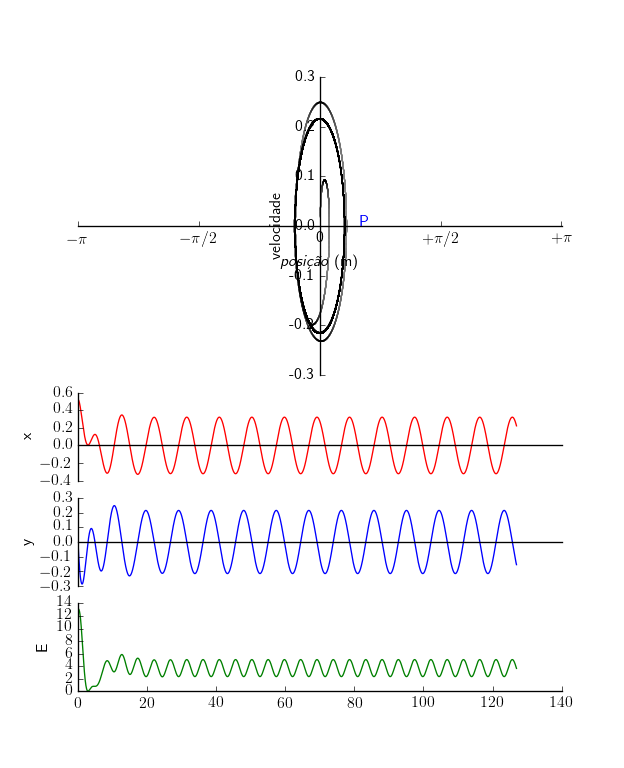
\includegraphics[width=6.24in,height=7.68in,keepaspectratio = false]{image1.png}
	
	\scriptsize Figura 2. Pendulo amortecido em movimento com uma força externa com A = 0.2,$\omega_f$ = 2/3 $\gamma$ = 0.5,l = 10. 
	
\end{center}

\begin{center}
	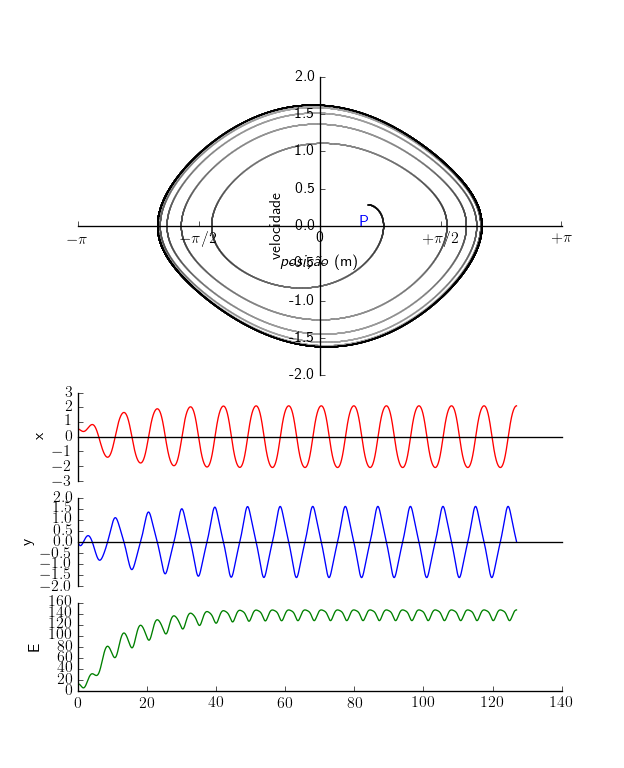
\includegraphics[width=6.24in,height=7.68in,keepaspectratio = false]{image2.png}
	
	\scriptsize Figura 3. Pendulo amortecido em movimento com uma força externa com A = 0.75,$\omega_f$ = 2/3 $\gamma$ = 0.5,l = 10. 
	
\end{center}

Mesmo partindo com A distintos o sistema se estabiliza em um ciclo limite, tanto na figura 1 como na 2, que é o atrator do sistema. Nesse caso o comportamento e dito como sistema periódico. 

O comportamento caótico é caracterizado pela grande sensibilidade às condições iniciais. O atrator não manifesta nenhuma regularidade:\textbf{ é estranho}.

\begin{center}
	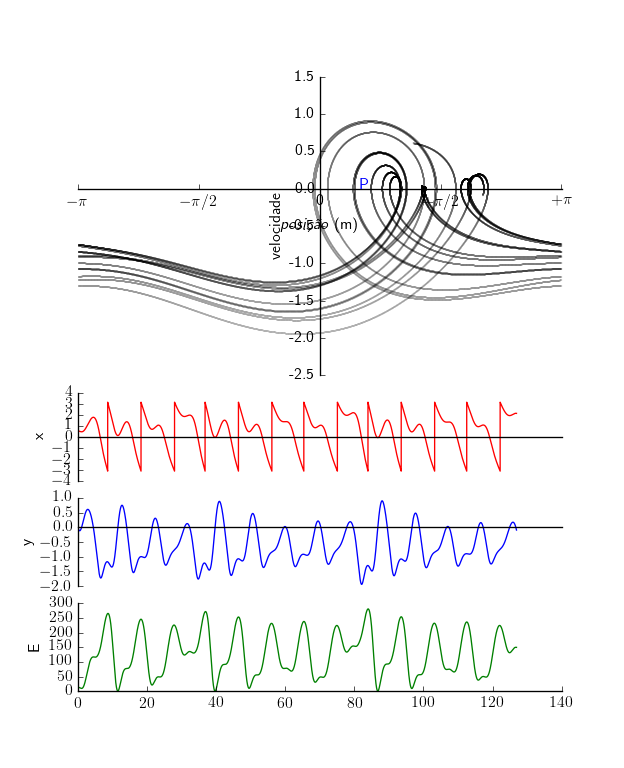
\includegraphics[width=6.24in,height=7.68in,keepaspectratio = false]{image3.png}
	
	\scriptsize Figura 4. Pendulo amortecido em movimento com uma força externa com A = 1.25,$\omega_f$ = 2/3 $\gamma$ = 0.5,l = 10, com \textbf{posição inicial de x = $\pi/6$}. 
	
\end{center}

\begin{center}
	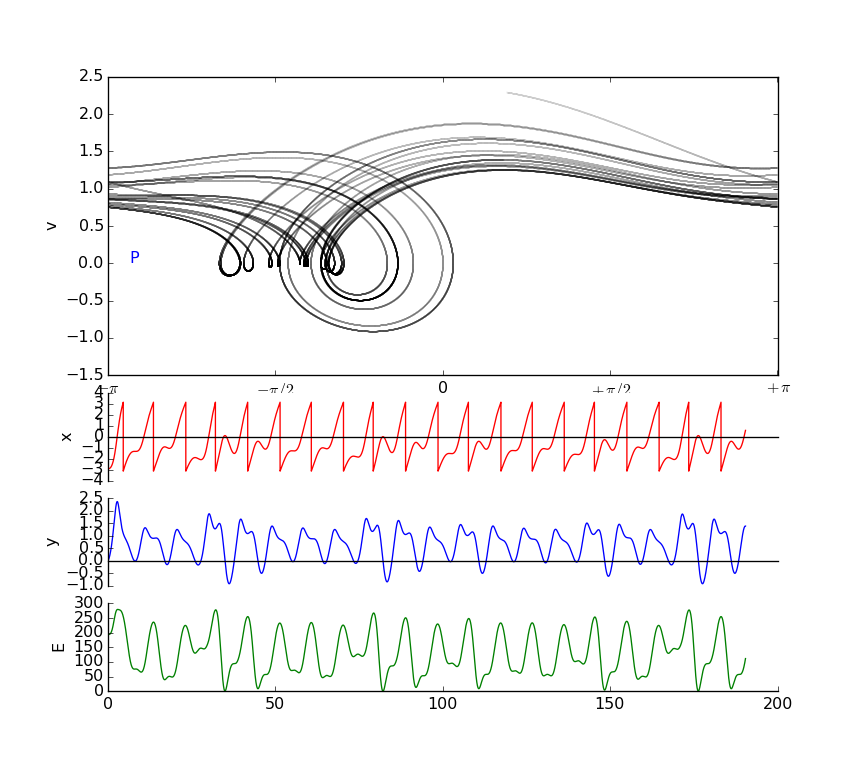
\includegraphics[width=6.24in,height=7.68in,keepaspectratio = false]{image6.png}
	
	\scriptsize Figura 5. Pendulo amortecido em movimento com uma força externa com A = 1.25,$\omega_f$ = 2/3 $\gamma$ = 0.5,l = 10, com \textbf{posição inicial de x = $\pi/6 - 10e-4$}. 
	
\end{center}

\begin{center}
	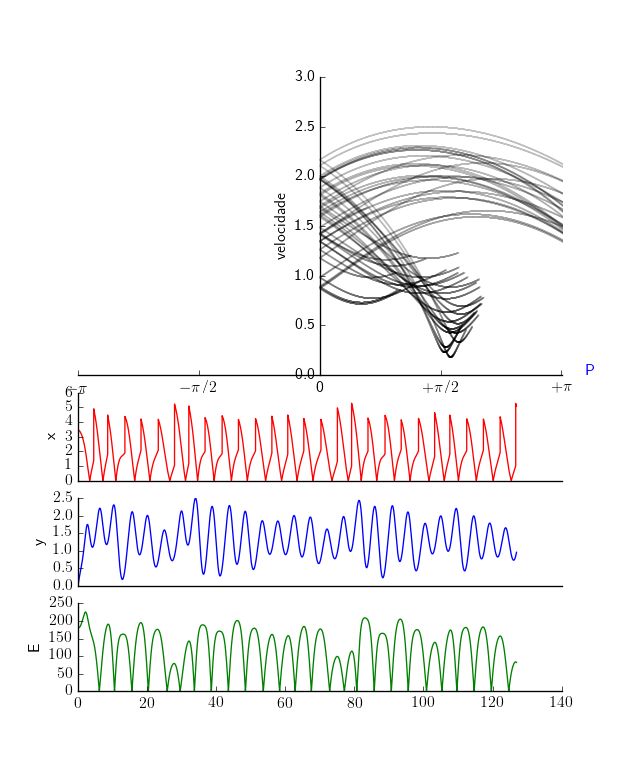
\includegraphics[width=6.24in,height=7.68in,keepaspectratio = false]{imageA.png}
	
	\scriptsize Figura 5. Pendulo amortecido com A = 1.25,$\omega_f$ = 2/3 $\gamma$ = 0.5,l = 10, com \textbf{posição inicial de x = $|x_1 - x_2| <1e-4$ e velocidade inicial v = $|v_1 - v_2| <1e-4$}. 
	
\end{center}

Devido a essa grande sensibilidade, dois pontos inicialmente próximos,em nosso casso a distancia entre os dois e de apenas míseros 10e-4m, estarão muito distantes após algum tempo. Esse efeito nos permite afirmar que os sistemas com comportamento caótico são imprevisíveis, ou seja, qualquer tentativa de previsão futura estará comprometida por pequenas imprecisões nas condições iniciais


\section{Conclus\~ao}

O pendulo forçado pode apresentar comportamento caótico para certos parâmetros em nosso caso para A > 1 ele não se estabiliza num ciclo limite: a trajetória no espaço de fase, que é tridimensional, nunca se cruza, para o caso de A < 1 o sistema aparenta se manter periódico. 
Em regime caótico apresenta uma grande sensibilidade às condições iniciais: pontos inicialmente próximos se afastam rapidamente. Essas características se aplicam a todos os sistemas com comportamento caótico.

\section{Referencia}

\noindent 

1)N. J. Giordano \& H. Nakanishi, Computational Physics, 2°ed, 2007

2)Sears \& Zemansky, F\'isica 2 Termodinâmica e ondas, 12°ed, 2008

3)M. A. Savi, "Din\^amica n\~ao-linear e caos", E-papers, Rio de Janeiro, 2006.

4)M\'etodo de Verlet, Wikip\'edia a enciclop\'edia livre, 2017

\end{document}

